\usepackage[utf8]{inputenc}
\usepackage[english,russian]{babel}
\usepackage[14pt]{extsizes}

%\usepackage{pscyr}
\usepackage{subfigure}
\usepackage{wrapfig}
\usepackage{cmap}
\usepackage{indentfirst}
\usepackage{autonum}
\usepackage{amsfonts}
\usepackage{amsmath}
\usepackage{amssymb}
\usepackage{amsthm}
\usepackage{upgreek}
\usepackage{graphicx}
\usepackage{listings}
\usepackage{multirow}
\usepackage{multicol}
\usepackage{dsfont}
\usepackage{graphicx}
\usepackage{caption}
\usepackage{setspace,amsmath}

\usepackage[unicode, pdftex]{hyperref}
\usepackage[left=30mm, top=20mm, right=15mm, bottom=20mm, footskip=10mm]{geometry}

\begin{document}
	\selectlanguage{russian}
\setcounter{page}{0}

\begin{center}
	\small{Министерство науки и высшего образования Российской Федерации}\\
	\small{Федеральное государственное бюджетное образовательное учреждение}\\
	\small{Высшего образования}\\
	\small{\textbf{«Северо-Осетинский государственный университет\\
			имени Коста Левановича Хетагурова»}}\\
	
	\hfill \break
	\hfill \break
	\hfill \break
	\hfill \break
	\hfill \break
	\hfill \break
	\hfill \break
	\hfill \break
	\hfill \break
	\hfill \break
	\hfill \break
	\hfill \break
	\hfill \break
	
	\normalsize{Дипломная работа}\\
	\large{\textbf{Seq2Seq - подход для реализации машинного перевода}}\\
	
	\hfill \break
	\hfill \break
	\hfill \break
	\hfill \break
	\hfill \break
	\hfill\break
\end{center}

\begin{flushright}
	\textbf{Выполнил:}\\
	Студент 4 курса направления:\\
	«Прикладная математика и информатика»\\
	\textit{Гамосов Cтанислав Станиславович \underline{\hspace{3cm}}}\\
\end{flushright}

\hfill

\begin{flushright}
	\textbf{Научный руководитель:}\\
	Кандидат физико-математических наук:\\
	\textit{Басаева Елена Казбековна \underline{\hspace{3cm}}}\\
\end{flushright}

\hfill

\begin{flushright}
	\textbf{Консультант}\\
	Старший преподаватель: \\
	\textit{Макаренко Мария Дмитриевна \underline{\hspace{3cm}}}\\
\end{flushright}

\normalsize{ \hspace{28pt}} \hfill \break
\begin{center} Владикавказ 2022 \end{center}
\thispagestyle{empty}
\clearpage
	\thispagestyle{empty}
\tableofcontents
\thispagestyle{empty}
\clearpage
\newtheorem{theorem}{Теорема}
	
	\section{Введение}
	
	На сегодняшний день перевод текстов становиться обыденностью и даже частью жизни. Крупные компании научили переводить не только текста в реальном времени, но и видео. Однако, буквально недавно исследователи почти столетие бились над алгоритмами машинного перевода и большая часть этого периода — без особых успехов.
    
    Само собой их наработки теперь лежат в основе всех современных систем обработки языка: от поисковиков до стиральных машин с голосовым управлением.
    
    В 1933 году советский ученый Пётр Троянский обращается в Академию наук СССР с изобретённой им «машиной для подбора и печатания слов при переводе с одного языка на другой». Машина была крайне проста: большой стол, печатная машинка с лентой и плёночный фотоаппарат. На столе лежали карточки со словами и их переводами на четырёх языках.
    
    Оператор брал первое слово из текста, находил карточку с ним, фотографировал её, а на печатной машинке набирал его морфологическую информацию: существительное, множественное число, родительный падеж.

    Её клавиши были модифицированы для удобства, каждая однозначно кодировала одно из свойств. Лента печатной машинки и плёнка камеры подавались параллельно, на выходе формируя набор кадров со словами и их морфологией:
    
    \begin{figure}[ht!]
		\centering
		\captionsetup{justification=centering}
		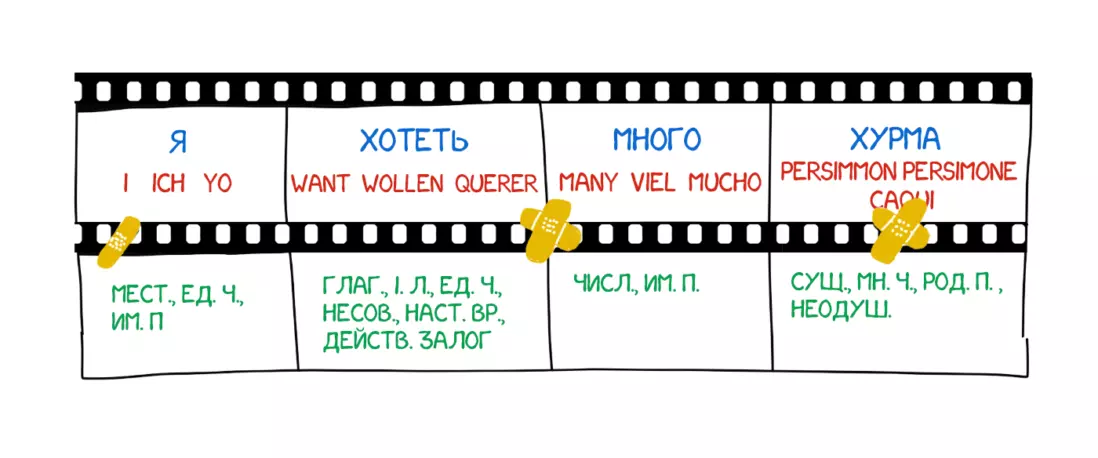
\includegraphics[height=60mm]{img/Машина_Троянского.png}
		\caption{Лента машины Троянского}
	\end{figure}
	
	Полученная лента отдавалась знающим конкретные языки лингвистам, которые превращали набор фотографий в связный литературный текст. Получается, чтобы переводить тексты, как оператору, так и лингвистам требовалось знать только свой родной язык.

    Машина Троянского впервые на практике реализовала тот самый «промежуточный язык» (interlingua), о создании которого мечтали ещё Лейбниц и Декарт.
    
    По классике в СССР изобретение признали ненужным, Троянский умер от стенокардии, 20 лет пытаясь доработать детище. Никто в мире так и не знал о машине, пока его патенты не откопали в архивах двое других советских учёных в 1956 году.
    
    Произошло это неслучайно. Они искали ответ на вызов холодной войны, ведь 7 января 1954 года в штаб-квартире IBM в Нью-Йорке произошёл Джорджтаунсий эксперимент. Компьютер IBM 701 впервые в мире автоматически перевёл 60 предложений с русского языка на английский.
    
    «Девушка, которая не понимает ни слова на языке Советов, набрала русские сообщения на перфокартах. Машинный мозг сделал их английский перевод и выдал его на автоматический принтер с бешеной скоростью - две с половиной строки в секунду - сообщалось в пресс-релизе компании IBM.
    
    \begin{figure}[ht!]
		\centering
		\captionsetup{justification=centering}
		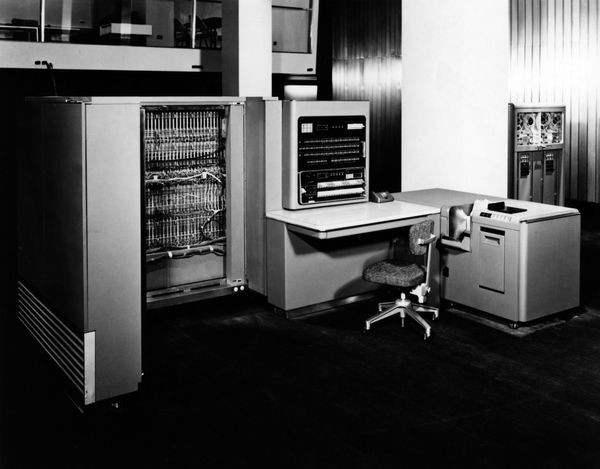
\includegraphics[height=60mm]{img/IBM 701.jpg}
		\caption{IBM 701}
	\end{figure}
    
    Газеты пестрили ликующими заголовками, но никто не говорил, что примеры для перевода были тщательно подобраны и протестированы, чтобы исключить любую неоднозначность. Для повседневного использования эта система подходила не лучше карманного разговорника.
    
    Современный машинный перевод работает на нейросетевых моделях. Некоторые редкие пары языков ещё используют более старую технологию статистического перевода, но все активно используемые в Яндекс.Переводчике языки, в том числе все языки России, работают на нейросетях.

    Основная идея обучения таких моделей - это прогонка множество пар параллельных текстов. Для перевода с входного на выходной язык такой парой будут предложение на входном и его перевод на выходном языке. Одна нейросеть — энкодер — преобразует входной текст в абстрактное представление, которое сохраняет свойства этого предложения в виде упорядоченного набора чисел. А другая нейросеть — декодер — генерирует на основе этого представления связный выходной текст.
	
	\textbf{Seq2Seq} - это семейство подходов машинного обучения, используемых для обработки естественного языка. Основные задачи для которого используется данные методы: нейронный перевод, субтитры к изображениям, разговорные модели и обобщение текста.
	
	Первоначальный алгоритм, который в процессе породил целое семейство методов, был разработан \textit{Google} для использования в машинном переводе. Как уже можно заметить за последнюю пару лет коммерческие системы стали удивительно хороши в  переводе - посмотрите, например, \textit{Google Translate}, \textit{Яндекс}-переводчик, переводчик \textit{DeepL}, переводчик \textit{Bing Microsoft}.
	
	Так же \textbf{Seq2Seq} технология несет в себе огромный потенциал, помимо привычного машинного перевода между естественными языками, вполне реализуем перевод между языками программирования (\textit{Facebook AI "Глубокое обучение переводу между языками программирования"}). Поэтому возможности применений такого рода подходов довольно велики. В связи с этим под машинным переводом будет подразумеваться любая задача \textbf{Seq2Seq}, если точнее, то перевод между последовательностями любой природы.
	
	\clearpage
	
	\section{Формализация задачи машинного перевода}
	
	Формально в задаче машинного перевода у нас есть входная последовательность $x_{1}, x_{2}, ... x_{m}$ и последовательность вывода $y_{1}, y_{2}, ... y_{n}$, само собой длинна данных последовательностей может отличатся. Саму процедуру \textit{перевода} можно рассматривать как нахождение искомой последовательности, которая является наиболее вероятной с учетом входных данных. Формально искомая последовательность, которая максимизирует условную вероятность $p(y|x): y^{'} = argmax[p(y|x)]$.
	
	Когда человеку известны уже два языка с которыми он работает, то уже при переводе можно сказать насколько хорошо справилась модель, является ли перевод естественным и насколько он приятен на слух. Однако такой вид анализа неприемлем для машины, поэтому нам стоит проанализировать уже имеющуюся функцию $p(y|x,\theta)$ с неким параметром $\theta$, а затем найти его $argmax$ для $y^{'} = argmax_{y}[p(y|x, \theta)]$.
	
	Прежде чем перейти к самой задачи перевода, нужно ответить на 3 вопроса:
	
	\begin{itemize}
		\item \textbf{Моделирование}: Как работает модель для $p(y|x, \theta)$?
		\item \textbf{Обучение}: Как найти параметр $\theta$?
		\item \textbf{Вывод}: Как понять, что текущий $y$ лучший?
	\end{itemize}
	
	\clearpage
	
	\section{Рекуррентные сети}
	
	\subsection{RNN - Recиrrent Neural Network}
	
	\textbf{Рекуррентные Нейронные Сети (Recиrrent Neural Network - RNN)} - это нелинейная динамическая система, которая сопоставляет последовательности с последовательностями. Основная философия заключается, в том что мысли обладают неким постоянством и напрямую зависят от прошлых умозаключений. 
	
	\begin{wrapfigure}{r}{0.25\textwidth}
		\centering
		\captionsetup{justification=centering}
		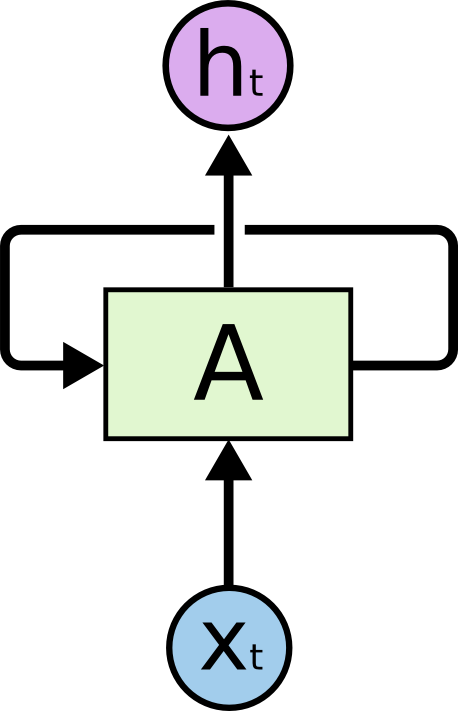
\includegraphics[height=45mm]{img/2.png}
		\caption{Рекуррентная нейронная сеть}
	\end{wrapfigure}
	
	RNN способны работать с последовательностями произвольной длины, а не с входными данными фиксированного размера. Это свойство как раз таки очень важно в контексте обработки естественных языков. Так же важное отличие таких сетей от обычных это понятие времени. Под ним подразумевается последовательность входных данных $x_t$, которая поступает на вход, и их выходная последовательность $y_t$, которые генерируются на основе дискретной входной последовательности. 
	
	Чтобы понять, что это значит, давайте проведем мысленный эксперимент. Скажем, вы делаете снимок шара, движущегося во времени.Допустим также, что вы хотите предсказать направление движения мяча. Таким образом, имея только ту информацию, которую вы видите на экране, как бы вы это сделали? Ну, вы можете пойти дальше и сделать предположение, но любой ответ, который вы придумали, был бы случайным предположением. Не зная, где находится мяч, у вас не будет достаточно данных, чтобы предсказать, куда он движется.Если вы запишете много снимков положения мяча подряд, у вас будет достаточно информации, чтобы сделать лучший прогноз.
	
	В результате получаемые последовательности могут быть конечной длины или бесконечно счетными. Таким образом, входную последовательность можно обозначить $x = (x_1, x_2, x_3, ... , x_t)$, а выходную последовательность как $y = (y_1, y_2, y_3, ... , y_t)$
	
	На схеме нейронная сеть $A$ принимает входное значение $x_t$ и возвращает значение $h_t$. Наличие обратной связи позволяет передавать информацию от одного шага сети к другому.
	
	Рекуррентную сеть можно рассматривать, как несколько копий одной и той же сети, каждая из которых передает информацию последующей копии. Вот, что произойдет, если мы развернем обратную связь:
	
	\begin{figure}[ht!]
		\centering
		\captionsetup{justification=centering}
		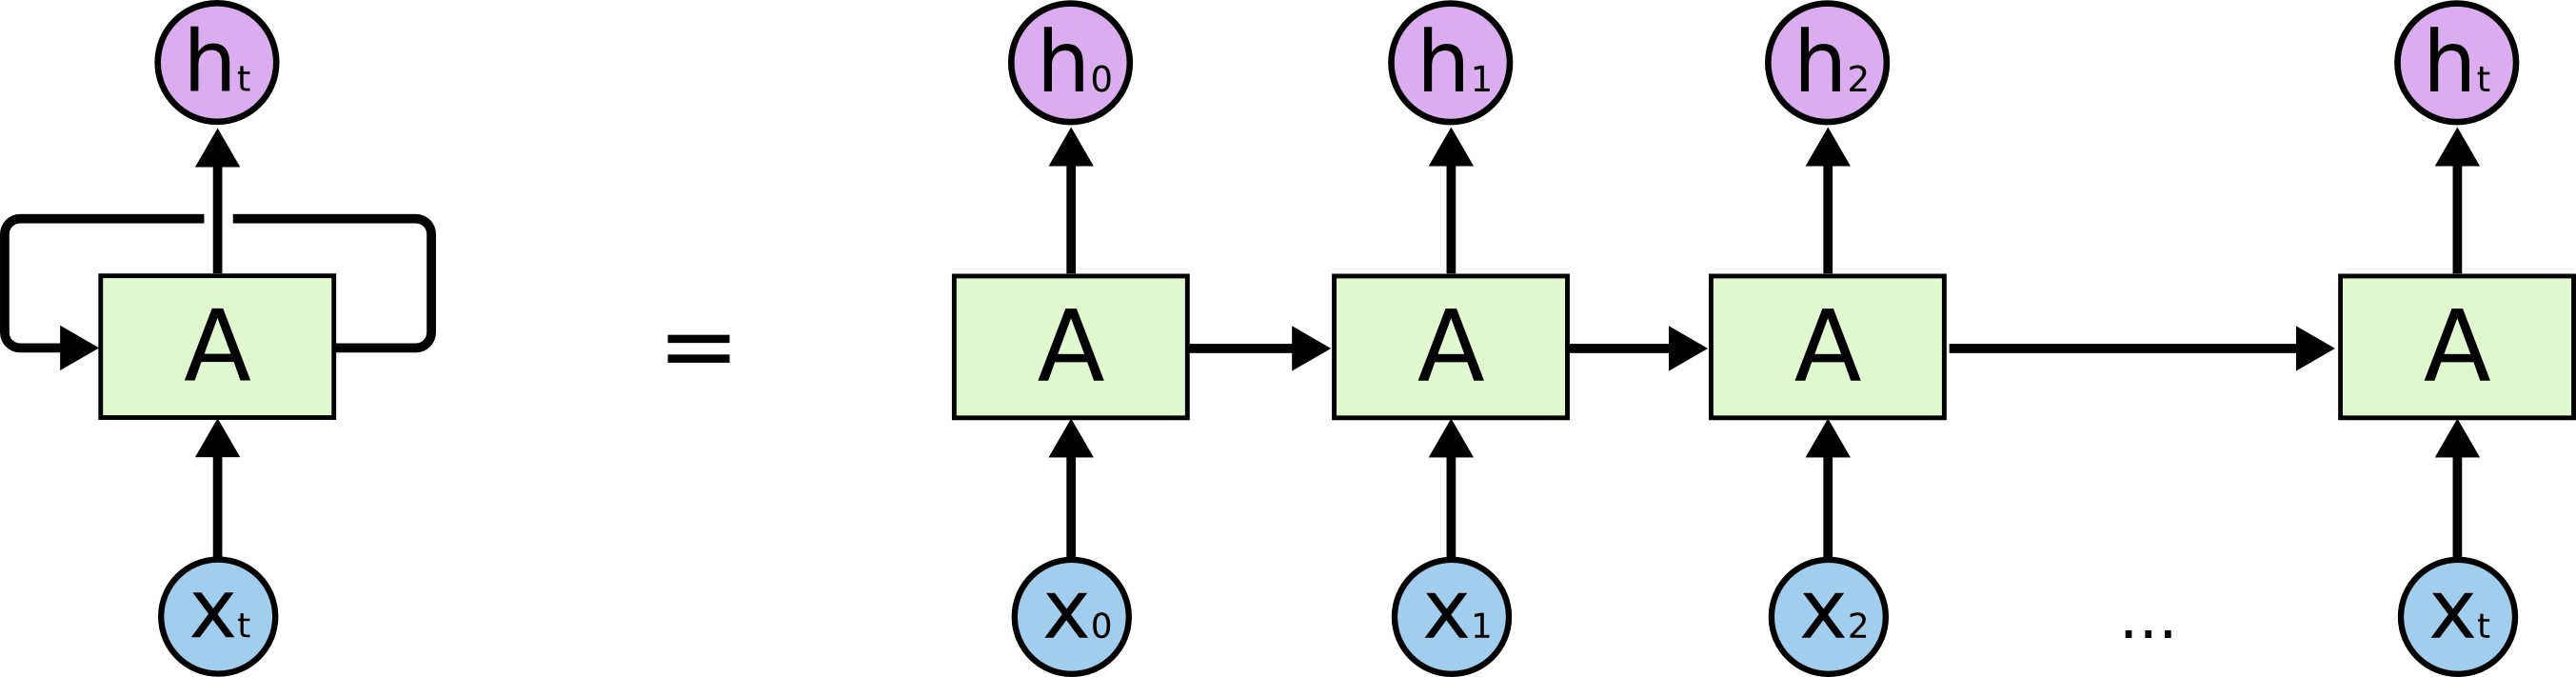
\includegraphics[height=40mm]{img/3.png}
		\caption{Развернутая рекуррентная нейронная сеть}
	\end{figure}
	
	То, что RNN напоминают цепи, может сказать нам лишь о том, что их довольно просто приложить к последовательностям. На данный этап RNN - самая естественная архитектура нейронных сетей для работы с данными таких типов.
	
	За последние несколько лет RNN с невероятным успехом применили к целому ряду задач: распознавание речи, языковое моделирование, распознавание изображений... Само собой в данной работе нас интересует, что такие сети довольно хорошо работают для задачи машинного перевода.
	
	\subsubsection{Elman Networks}
	
	Для большей понимания рекуррентных сетей рассмотрим, пару архитектур. Нейронная сеть Элмана состоит из трёх слоев: $x, y, h$. Дополнительно к сети добавлен набор \textbf{контекстных блоков} - $c$. Скрытый слой $h$ соединён с контекстными блоками с фиксированным весом, равным единице. В данном случае веса равны единицам, однако это не всегда так. В свою очередь \textbf{вес} - это связь между вершинами, которая несет в себе значение, характеризующее важность, передаваемого значения, проходящего через данное ребро. 
	
	Для пары узлов $i$ (узел входного слоя) и $j$ (узел скрытого слоя) присутствует собственный вес $w_{i,j}$. Легче всего это представить как матрицу смежности $W$, где на пересечение $i$ строки и $j$ столбца находятся числа отвечающие за вес. Такая же матрица только для скрытого слоя в выходной слой будем обозначать $U$. 
	
	С каждым шагом времени на вход $x$ поступает информация, которая проходит прямой ход к выходному слою $y$v в соответствии с правилами обучения. Фиксированные обратные связи сохраняют предыдущие значения скрытого слоя $h$ в контекстных блоках $c$(до того как скрытый слой поменяет значение в процессе обучения). Таким способом сеть сохраняет своё состояние, что может использоваться в предсказании последовательностей, выходя за пределы мощности многослойного перцептрона.
	
	\begin{table}[h]
		\centering
		\begin{tabular}{|c|} 
			\hline
			\textbf{Elman Networks}  \\ 
			\hline
			$ h_{t} = \sigma_{h}(W_h x_t + U_h h_{t - 1} + b_h) $ \\ 
			$ y_{t} = \sigma_{y}(W_y h_t + b_y) $ \\
			\hline
		\end{tabular}
	\end{table}
	\begin{tabbing}
		$x_t$ - вектор входного слоя        \\
		$h_t$ - вектор срытого слоя         \\
		$y_t$ - вектор выходного слоя       \\
		$W$, $U$ и $b$ - матрицы и вектор параметров       \\
		$\sigma_h$ и $\sigma_y$ - функции активации
	\end{tabbing}
	
	\textbf{Функция активации} $\sigma$ в свою очередь является абстракцией, представляющей скорость возбуждения нейрона. Список функций активации, которых чаще всего используют:
	
	\begin{table}[h]
		\centering
		\begin{tabular}{|l|l|} 
			\hline
			Функция Хевисайда       &   
			$ H(x) = 
			\begin{cases}
				0, & x < 0 \\
				1, & x >= 0 \\
			\end{cases}$ \\ 
			\hline
			Cигмоида                &  $\sigma(x) = \frac{1}{1 + e^{-x}}$ \\ 
			\hline
			Гиперболический тангенс &  $tanh(x) = \frac{e^x - e^{-x}}{e^x + e^{-x}}$ \\ 
			\hline
			Линейный выпрямитель    &  $ReLU(x) = max(0, x)$ \\
			\hline
		\end{tabular}
	\end{table}
	
	Некоторые желательные свойства функций активации:
	
	\begin{itemize}
		\item \textit{Нелинейность}
		\item \textit{Непрерывная дифференцируемость}
		\item \textit{Ограниченность области значений}
		\item \textit{Монотонность}
		\item \textit{Гладкость функции с монотонной производной}
		\item \textit{Аппроксимировать тождественной функцию около начала координат}
	\end{itemize}
	
	\subsubsection{Jordan Networks}
    
    Так же существует вторая архитектура RNN нейронная сеть Джордана. Подобна сети Элмана, но контекстные блоки связаны не со скрытым слоем, а с выходным слоем. Контекстные блоки таким образом сохраняют своё состояние. Они обладают рекуррентной связью с собой.
    
	\begin{table}[h]
			\centering
			\begin{tabular}{|c|} 
				\hline
				\textbf{Jordan Networks}  \\ 
				\hline
				$	h_{t} = \sigma_{h}(W_h x_t + U_h y_{t - 1} + b_h) $  \\
				$	y_{t} = \sigma_{y}(W_y h_t + b_y) $ \\
				\hline
			\end{tabular}
	\end{table}
	
	\begin{tabbing}
		$x_t$ - вектор входного слоя        \\
		$h_t$ - вектор срытого слоя         \\
		$y_t$ - вектор выходного слоя       \\
		$W$, $U$ и $b$ - матрицы и вектор параметров       \\
		$\sigma_h$ и $\sigma_y$ - функции активации
	\end{tabbing}
	
	\begin{figure}[ht!]
		\centering
		\captionsetup{justification=centering}
		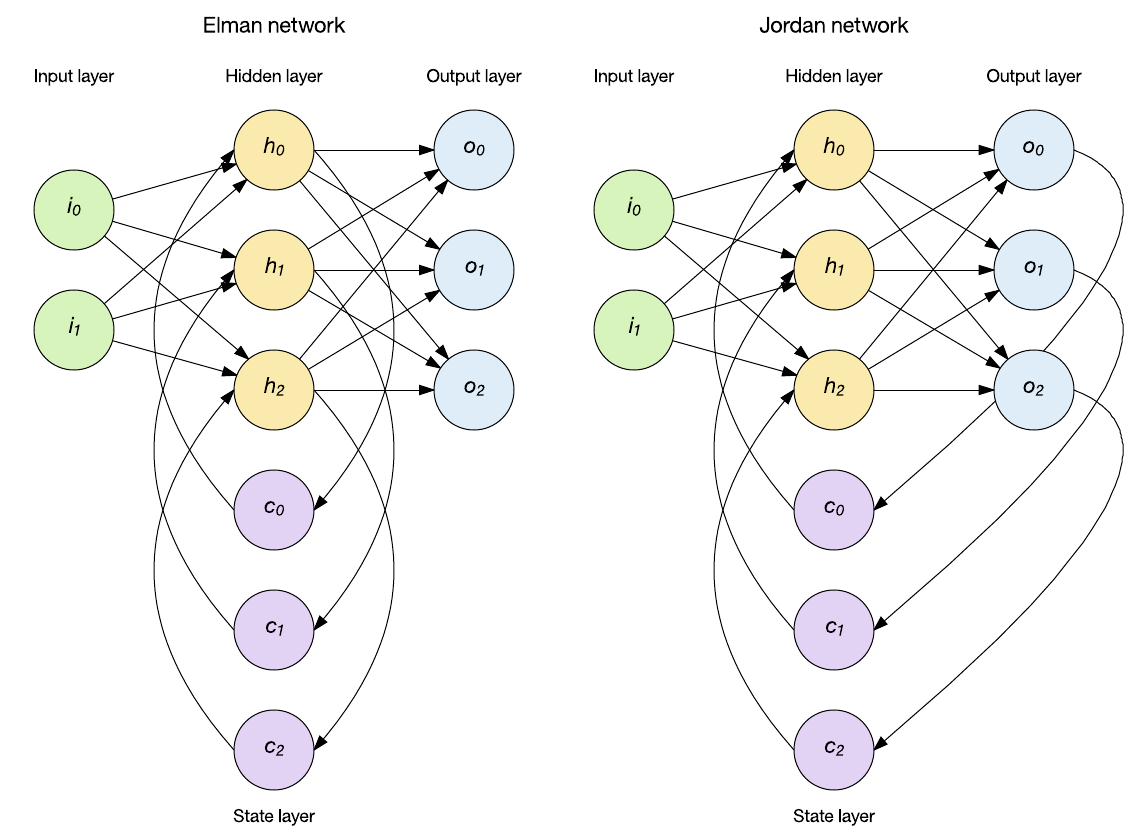
\includegraphics[width=140mm]{img/RNN.png}
		\caption{Схемы архиетектур рекуррентных нейронных сетей}
	\end{figure}
	
	\subsection{Проблема долговременных зависимостей}
	
	Одна из привлекательных идей RNN состоит в том, что они потенциально умеют связывать предыдущую информацию с текущей задачей. Как это было на примере полета шарика. Однако действительно ли RNN предоставляют нам такую возможность? Это зависит от некоторых обстоятельств.

	Во время работы с RNN было замечено, что случае, когда дистанция между актуальной информацией и местом, где она понадобилась, велика, то сети могут могут забыть нужную информацию из прошлого. Долгосрочные зависимости плохо воспринимаются обычными рекурсивными сетями, потому что градиенты имеют тенденцию либо исчезать (большую часть времени), либо взрываться (редко, но с серьезными последствиями). Это затрудняет метод оптимизации на основе градиента не только из-за различий в величинах градиента, но и из-за того, что эффект долгосрочных зависимостей скрыт эффектом краткосрочных зависимостей. 
	
	Существовало два доминирующих подхода, с помощью которых многие исследователи попытались уменьшить негативные последствия этой проблемы. Один из таких подходов заключается в разработке лучшего самообучающийся алгоритм, чем простой стохастический градиентный спуск.
	
	Другой подход, который нас больше интересует, заключается в разработке более сложной функции активации, чем обычные функции что применялись ранее. Самая ранняя попытка в этом направлении привела к появлению функции активации или повторяющегося блока, называемого блоком долговременной кратковременной памяти (LSTM)[2]. Более современный тип повторяющейся единицы, к которому мы относимся как к закрытой повторяющейся единице (GRU)[3]. Было показано, что некоторые из этих повторяющихся блоков хорошо справляются с задачами, требующими учета долгосрочных зависимостей.
	
	\subsection{GRNN - Gated Recurrent Neural Networks}
	\subsubsection{LSTM - Long Short-Term Memory}
	
	Сети долгой краткосрочной памяти (LSTM) - особая разновидность архитектуры RNN, способная к обучению долговременным зависимостям. Они были представлены Зеппом Хохрайтер и Юргеном Шмидхубером в 1997[2]. Они прекрасно решают целый ряд разнообразных задач и в настоящее время широко используются. Любая рекуррентная нейронная сеть имеет форму цепочки повторяющихся модулей нейронной сети. В обычной RNN структура одного такого модуля очень проста, например, он может представлять собой один слой с функцией активации $tanh$. 
	
	\begin{figure}[ht!]
		\centering
		\captionsetup{justification=centering}
		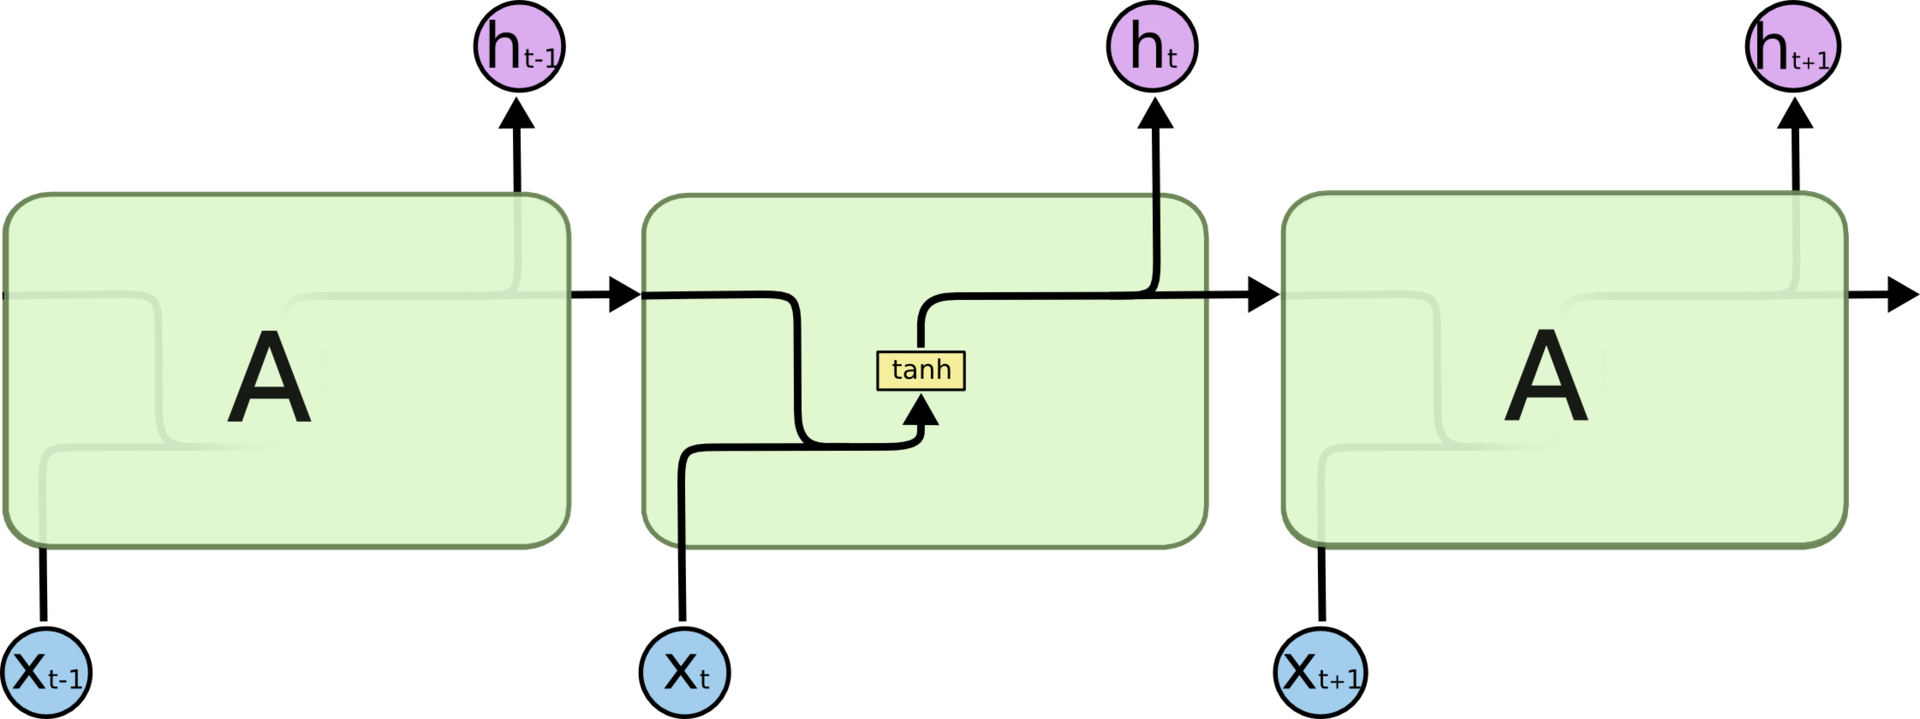
\includegraphics[height=40mm]{img/RNN Chain.png}
		\caption{Повторяющийся модуль в стандартной RNN состоит из одного слоя}
	\end{figure}
	
	Структура LSTM также напоминает цепочку, но модули выглядят иначе. Вместо одного слоя нейронной сети они содержат целых четыре, и эти слои взаимодействуют особенным образом. 
	
	\begin{figure}[ht!]
		\centering
		\captionsetup{justification=centering}
		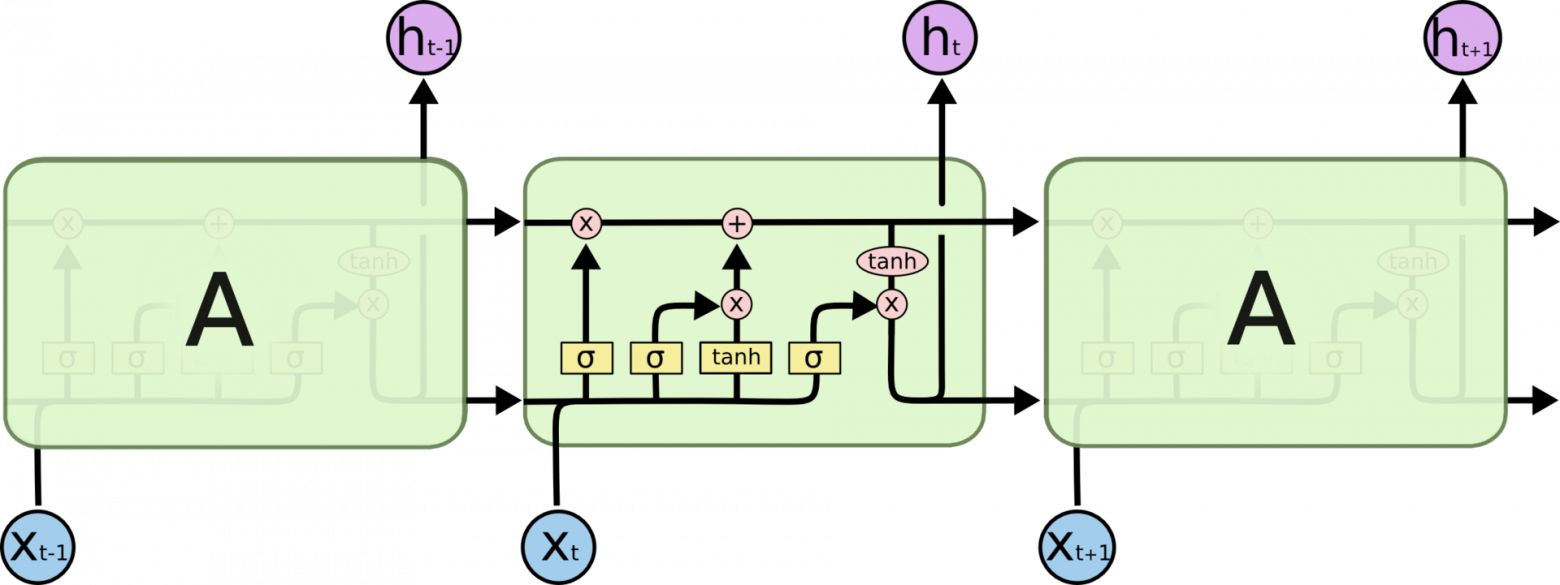
\includegraphics[height=40mm]{img/LSTM Chain.png}
		\caption{LSTM сети состоит из четырех взаимодействующих слоев}
	\end{figure}
	
	Ключевой компонент LSTM – это состояние ячейки (cell state) – горизонтальная линия, проходящая по верхней части схемы
	
	Состояние ячейки напоминает конвейерную ленту. Она проходит напрямую через всю цепочку, участвуя лишь в нескольких линейных преобразованиях. Информация может легко течь по ней, не подвергаясь изменениям.
	
	\begin{figure}[ht!]
		\centering
		\captionsetup{justification=centering}
		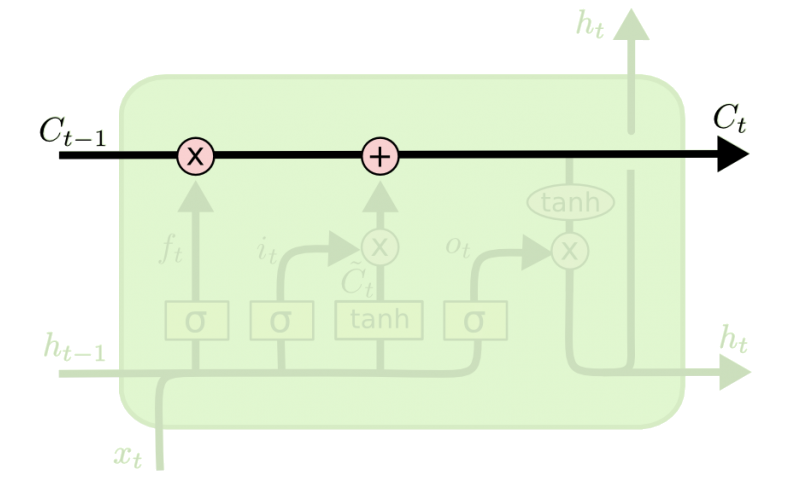
\includegraphics[height=40mm]{img/LSTM 1.png}
	\end{figure}
	
	Тем не менее, LSTM может удалять информацию из состояния ячейки; этот процесс регулируется структурами, называемыми фильтрами (gates). Фильтры позволяют пропускать информацию на основании некоторых условий. Они состоят из слоя сигмоидальной нейронной сети и операции поэлементного умножения.
	
	Сигмоидальный слой возвращает числа от нуля до единицы, которые обозначают, какую долю каждого блока информации следует пропустить дальше по сети. Ноль в данном случае означает \textit{не пропускать ничего}, единица - \textit{пропустить все}.

    \textbf{Пошаговая работа LSTM:}
    
    Первый шаг в LSTM - определить, какую информацию можно выбросить из состояния ячейки. Это решение принимает слой на котором применяем сигмойду, называемый \textit{слоем фильтра забывания} (forget gate layer). Он смотрит на $h_{t-1}$ и $x_t$ и возвращает число от 0 до 1 для каждого числа из состояния ячейки $C_{t-1}$.
    
    \begin{figure}[ht!]
		\centering
		\captionsetup{justification=centering}
		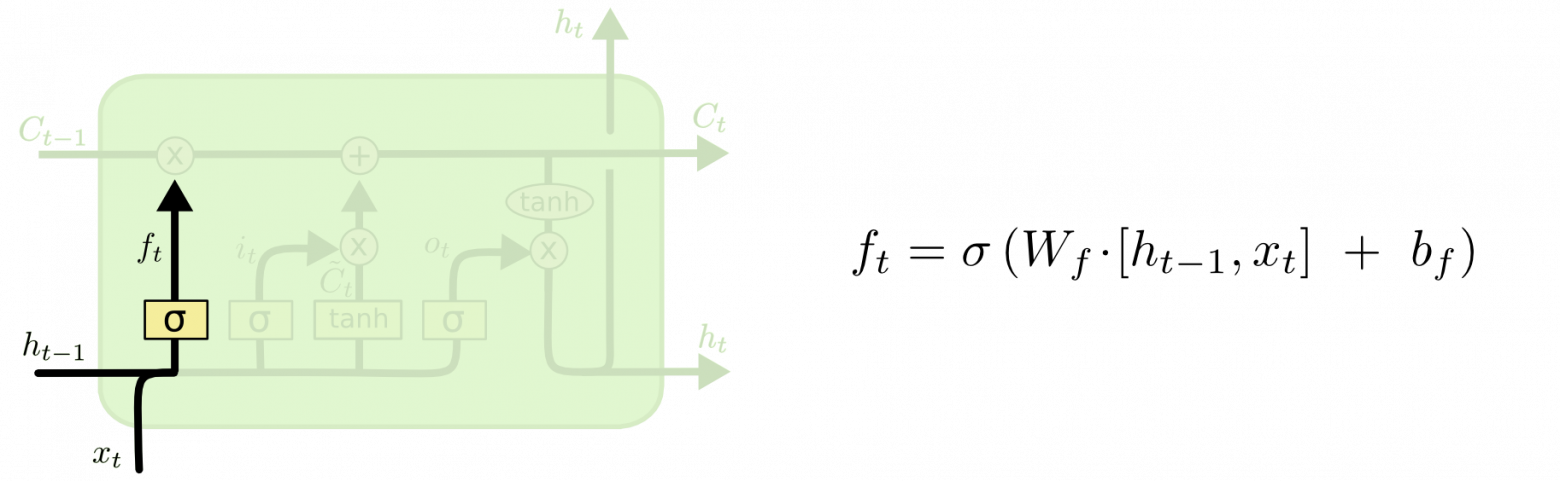
\includegraphics[height=40mm]{img/LSTM_step1.png}
	\end{figure}
	
	Следующий шаг - решить, какая новая информация будет храниться в состоянии ячейки. Этот этап состоит из двух частей. Сначала сигмоидальный слой под названием \textit{слой входного фильтра} (input layer gate) определяет, какие значения следует обновить. Затем действует функция активации tanh, в результате пролучаем вектор новых значений-кандидатов $\tilde{c}_t$, которые можно добавить в состояние ячейки.
    
    \begin{figure}[ht!]
		\centering
		\captionsetup{justification=centering}
		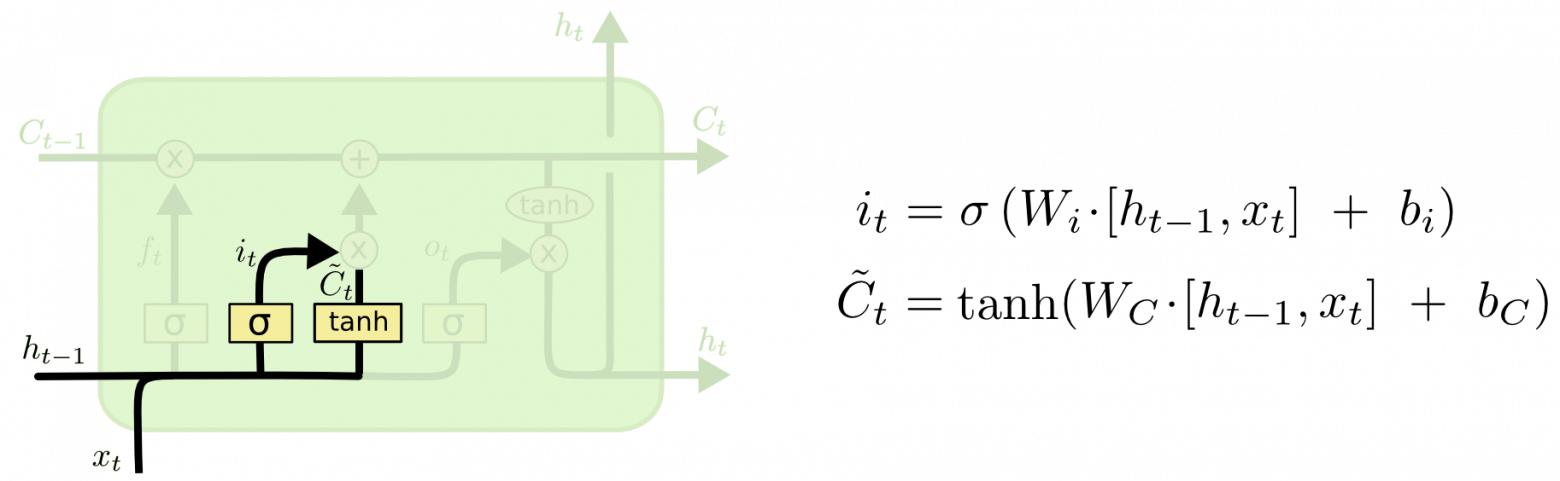
\includegraphics[height=40mm]{img/LSTM_step2.png}
	\end{figure}
	
    После всего этого нужно заменить старое состояние ячейки $c_{t-1}$ на новое состояние $c_t$.
    
    Необходимо умножить старое состояние на $f_t$, забывая то, что мы решили забыть. Затем прибавляем $i_t*\tilde{c}_t$. Это новые значения-кандидаты, умноженные на $t$ – на сколько мы хотим обновить каждое из значений состояния.
    
    \begin{figure}[ht!]
		\centering
		\captionsetup{justification=centering}
		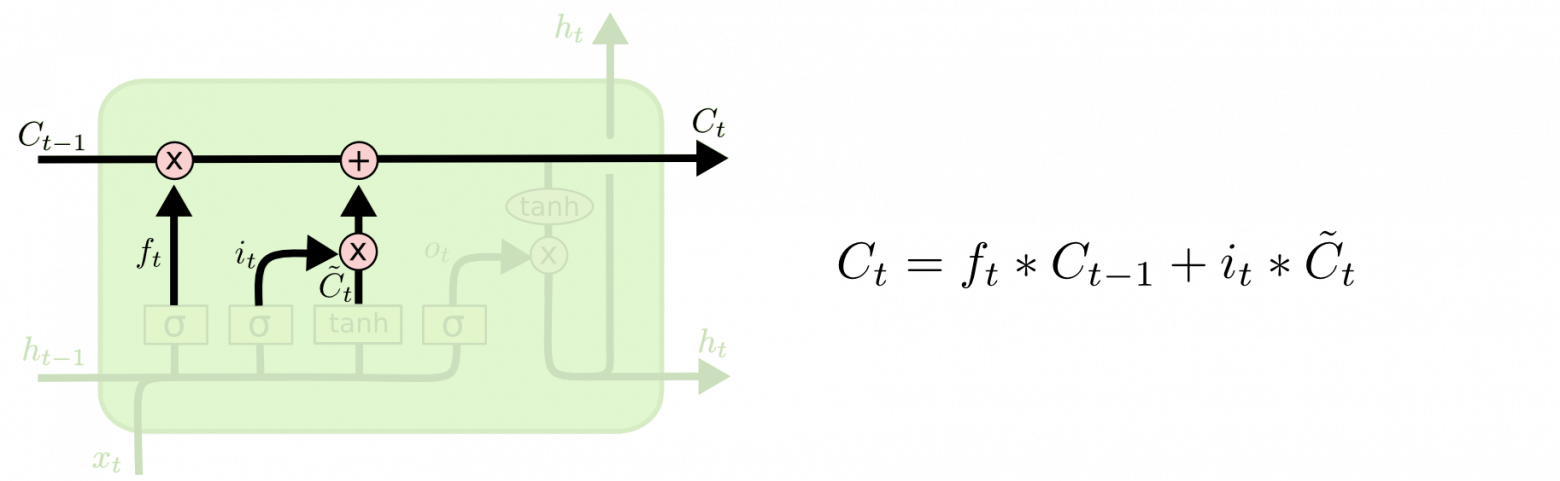
\includegraphics[height=40mm]{img/LSTM_step3.png}
	\end{figure}
	
	Наконец, нужно решить, какую информацию мы хотим получать на выходе. Выходные данные будут основаны на нашем состоянии ячейки, к ним будут применены некоторые фильтры. Сначала мы применяем функцию активации сигмойд, которая решает, какую информацию из состояния ячейки мы будем выводить. Затем значения состояния ячейки проходят через активацию tanh, чтобы получить на выходе значения из диапазона от -1 до 1, и перемножаются с выходными значениями сигмоидального слоя, что позволяет выводить только требуемую информацию.

    \begin{figure}[ht!]
		\centering
		\captionsetup{justification=centering}
		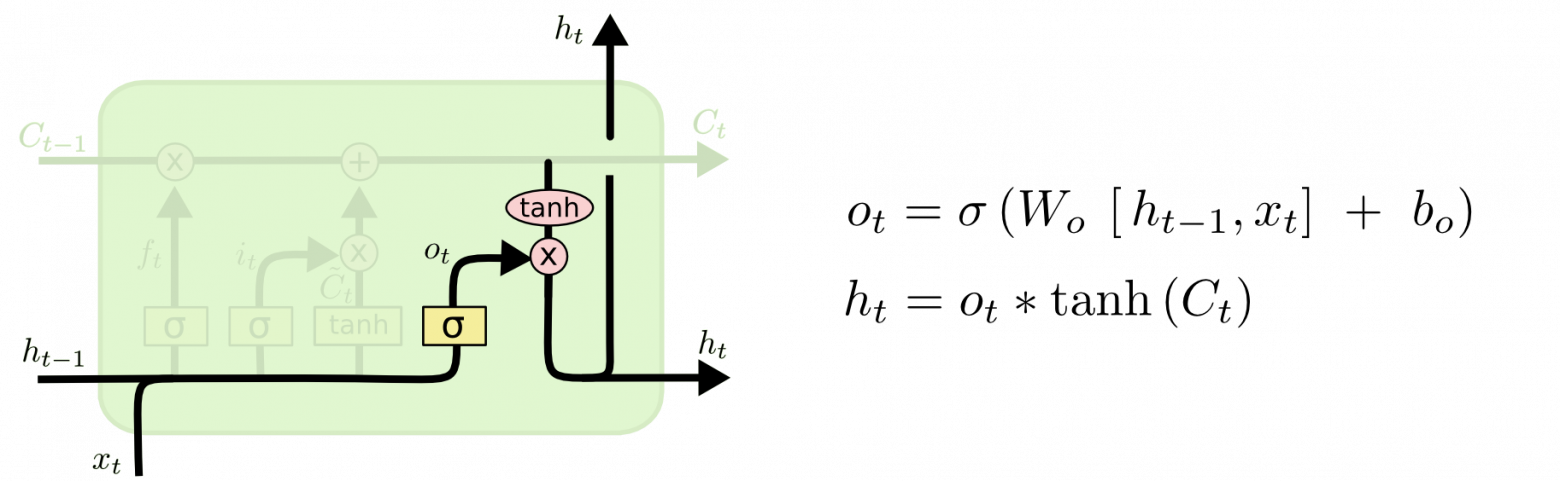
\includegraphics[height=40mm]{img/LSTM_step4.png}
	\end{figure}
	
	В отличие от традиционных рекуррентных сетей, которые перезаписывают свое содержимое на каждом шаге времени, блок LSTM способен решать, следует ли сохранять существующую память или нет с помощью введенных элементов. Интуитивно понятно, что если модуль LSTM обнаруживает важную функцию из входной последовательности на ранней стадии, он легко переносит эту информацию на большие расстояния, следовательно, фиксируя потенциальные зависимости.
	
	\subsubsection{GRU - Gated Recurrent Unit}
	
	\textbf{GRU - Gated Recurrent Unit} Управляемые рекуррентные блоки была предложена в 2014[3], чтобы каждая рекуррентная единица могла адаптивно фиксировать зависимости разных временных масштабов. Аналогично блоку LSTM, GRU имеет
	фильтра, которые модулируют поток информации внутри блока, однако, не имея отдельных ячеек памяти.
	
    GRU избавилось от ячеек состояния и использует скрытое состояние для передачи информации. Эта архитектура также имеет только два фильтра, фильтр сброса и фильтр обновления.
    
    \textit{Слой фильтра обновления} (update layer gate) элемент обновления действует аналогично слоям входного и выходного фильтра в LSTM. Он решает, какую информацию выбросить и какую новую информацию добавить.
    
    \textit{Слой фильтра сброса} (reset layer gate) - это еще один элемент, который используется для определения того, сколько прошлой информации следует забыть.
    У GRU меньше тензорных операций, следовательно, их обучение этой архитектуры немного быстрее, чем у LSTM. Нет явного победителя, который из них лучше. Исследователи и инженеры обычно используют и то, и другое, чтобы определить, какой из них лучше подходит для их варианта использования.
    
    \begin{figure}[ht!]
		\centering
		\captionsetup{justification=centering}
		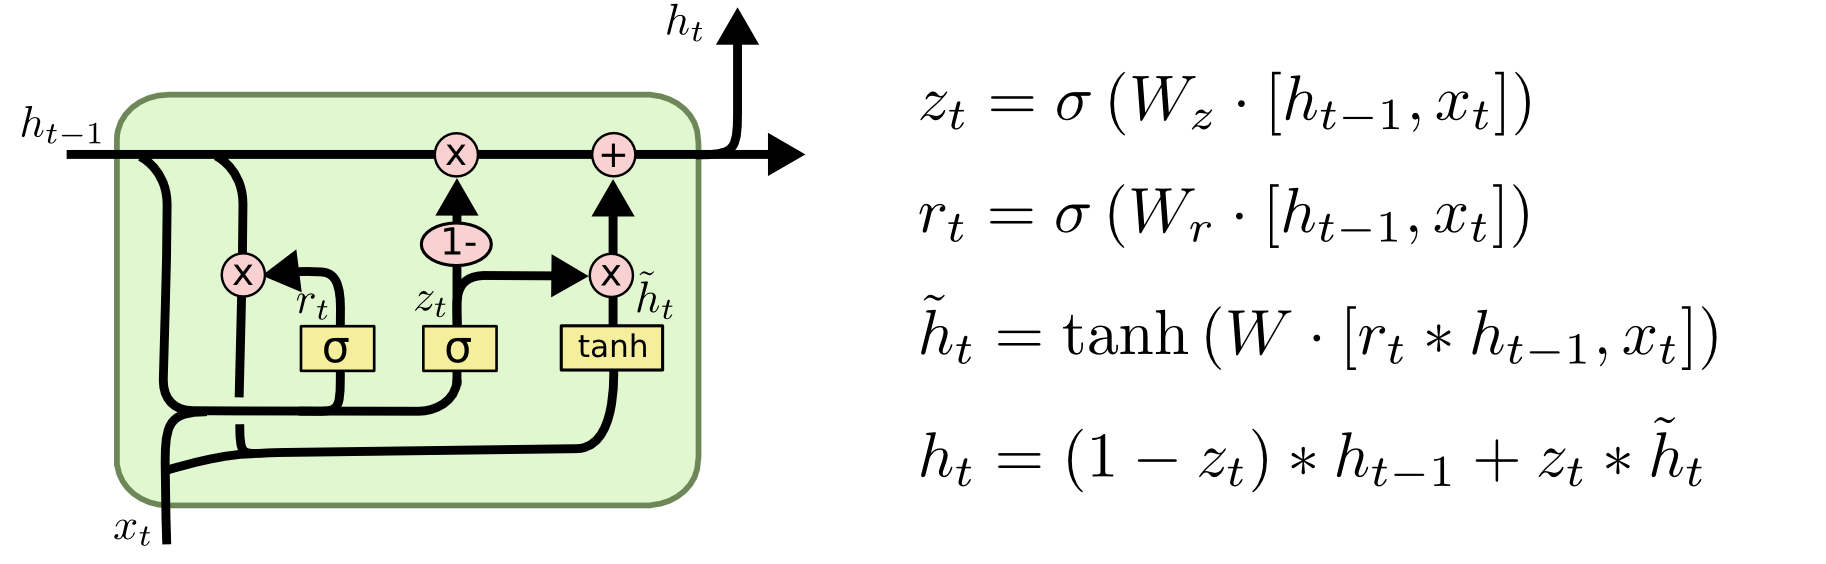
\includegraphics[height=45mm]{img/GRU.png}
	\end{figure}
	
	\clearpage
 	
 	\section{Построение модели Seq2Seq}
	
	Наиболее интересная модель для задачи машинного перевода \textbf{Seq2Seq} являются модель \textbf{Encoder-Decoder}, в которой обычно используют \textbf{рекуррентные нейронные сети} (\textbf{RNN}) для кодирования исходной последовательности в один вектор. В дальнейшем будем называть этот единственный вектор - \textbf{вектором контекста}. Можно думать о векторе контекста как об абстрактном представлении всего входного предложения. В целом этот вектор контекста можно назвать набором образов сущностей с образами взаимоотношений между ними. 

	Однако с полученный вектор необходимо преобразовать в предложение. В таком случаее используется вторая RNN - декодер, которая учится выводить целевое выходное предложение, генерируя его слово за словом.
	
	\begin{figure}[ht!]
		\centering
		\captionsetup{justification=centering}
		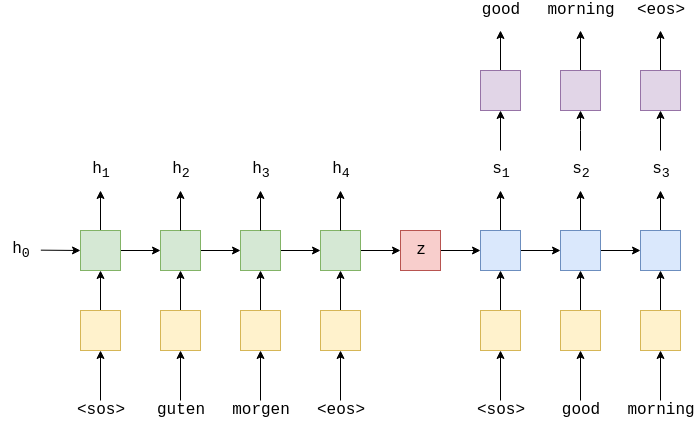
\includegraphics[height=80mm]{img/encoder-decoder-img-1.png}
	\end{figure}
	
	На вход такой модели вводится предложение, «guten morgen», проходит через слой эмбеддинга. На схеме желтый блок, служит для сопоставления элементов предложения, к числовому вектору. Полученный вектор отправляется в кодировщик (зеленый блок).
	
	Для однозначности конца и начала предложения в имеющуюся последовательность добавляются токены начало последовательности (<sos> - start of sequence) и конец последовательности (<eos> - end of sequence). 
	
	На каждом временном шаге на вход в RNN кодировщика подаётся как эмбеддинг-версия текущего слова $e(x_t)$ которая порождена слоем эмбеддинга $e$, так и скрытое состояние из предыдущего временного шага, $h_{t-1}$. На выход RNN кодировщика подаёт новое скрытое состояние $h_t$. Здесь мы можем думать о скрытом состоянии как о векторном представлении предложения. RNN кодировщика может быть представлена как функция $EncoderRNN$ от переменных $e(x_t)$ и $h_{t-1}$
	
	$$
	    h_t = EncoderRNN(e(x_t), h_{t-1})
	$$
	
	В данном контексте под RNN может подразумеваться любая рекуррентная сеть. Например: LSTM или GRU.
	
	Последовательность $X = {x_1, x_2, ..., x_t}$ где $x_i$ - это слова входной последовательности и токены начала и конца. Начальное скрытое состояние, $h_0$ обычно либо инициализируется нулями.

    После того как последнее слово $x_t$ было передано в RNN через слой эмбеддинга, мы используем конечное скрытое состояние $h_t$ как вектор контекста, то есть $c = h_t$. Это векторное представление всего исходного предложения.
    
    Теперь вектор контекста $c$, можно декодировать, чтобы получить выходное предложение. Как и в предыдущем случае, добавляются токены начала и конца последовательности к целевому предложению. На каждом временном шаге входом в RNN декодера (синий блок) является эмбеддинг текущего слова $d(y_t)$, а также скрытое состояние из предыдущего временного шага $s_{t-1}$, где начальное скрытое состояние декодера $s_0$, является вектором контекста, $s_0 = c$. Иными словами начальное скрытое состояние декодера является окончательным скрытым состоянием кодера. Таким образом, аналогично кодеру, мы можем представить декодер как функцию от переменных $d(y_t)$ и $s_{t-1}$:
    
    $$
	    s_t = DecoderRNN(d(x_t), s_{t-1})
	$$
	
	Хотя слой эмбеддинга входа $e$ и слой эмбеддинга выхода $d$ оба показаны жёлтым цветом, они представляют собой два разных слоя со своими собственными параметрами.

    В декодере нам нужно перейти от скрытого состояния к фактическому слову, поэтому на каждом временном шаге мы используем $s_t$ для распознавания того, что мы считаем следующим словом в последовательности $\hat{y}_t$ (фиолетовый блок).

    $$
        \hat{y}_t = f(s_t)
    $$
    
    Слова в декодере всегда генерируются одно за другим, по одному за один временной шаг. Поэтому всегда используем <sos> в качестве первого слова $y_1$ для ввода в декодер, но для последующих слов для ввода $y_{t>1}$, иногда используются фактическое, истинное следующее слово в последовательности $y_t$, и иногда берется слово, предложенное нашим декодером $\hat{y}_{t-1}$. Такой метод обучения называется обучением с принуждением.

    При обучении модели всегда известно, сколько слов в целевом предложении, поэтому генерирование слов останавливается, как только набирается нужное количество. Во время рабочего вывода обычно генерируют слова до тех пор, пока модель не выдаст токен окончания последовательности или после того, как будет сгенерировано определенное количество слов.
    
    В дальнейшем предсказанное предложение $\hat{Y} = { \hat{y}_1, \hat{y}_2, ..., \hat{y}_t }$, сравнивается с нашим фактическим целевым предложение, $Y = { y_1, y_2, ..., y_t }$, для расчета потерь. Затем полученное значение используется для обновления всех параметров обучаемой модели.

    \clearpage
	
	\subsection{Encoder}
	
	\clearpage
	
	\subsection{Decoder}
	
	\clearpage
	
	\section{Код}
	
	\begin{minted}[fontsize=\footnotesize]{python}
language_data = pd.DataFrame(columns=['Source','Target'])
language_data['Source'] = source_word
language_data['Target'] = target_word
	\end{minted}
	
	Модель Seq2Seq хочет, чтобы вся входная последовательность была одинаковой длины. Один из способов добиться этого - мы вычисляем длину каждого предложения как на входном языке, так и на выходном языке, а затем выбираем максимальную длину, то есть самое длинное предложение на обоих языках. 
	
	Поскольку машины понимают только числа, а не текст, нужен способ преобразовать входную текстовую последовательность в числа, и одним из таких способов является индексация слов предложений. Мы можем выполнить эту индексацию, используя библиотеку \textbf{Keras} и ее метод \textbf{Tokenizer}. Также необходимо учитывать размер словарного запаса как входных, так и выходных последовательностей, это в дальнейшем потребуется при создании входных данных для обучения модели.

    Итак, как вы можете видеть, была создана функция \mintinline{c++}{generator_batch}, которая принимает три параметра \mintinline{c++}{X, Y, batch_size}. Теперь первое, что есть в функции, - это цикл \mintinline{c++}{while}, и этот цикл настроен на то, чтобы всегда выполняться. Мы запускаем цикл \mintinline{c++}{for} от 0 до длины нашего \mintinline{c++}{X} (тренировочные данные), который увеличивается на \mintinline{c++}{batch_size}, который мы задаем сами. 
    
    \mintinline{c++}{encoder_data_input, decoder_data_input, decoder_target_input} - внутренние переменные цикла, которые стоит расмотреть по отдельности. 
	
	Я создал матрицу нулей, имеющих количество строк, равное \mintinline{c++}{batch_size}, и столбцов, равных \mintinline{c++}{max_length_english} для encoder'а, и аналогично для decoder'а. Можно увидеть целевые данные decoder'а, они расфасованы по трем переменным, потому что выходные данные decoder'а являются трехмерными. Однако, decoder - это то, что дает переведенное предложение в качестве вывода. Отсюда возникает вопрос почему также был создан ввод декодера? Это сделано для ускорения обучение, и так же этот метод называется \textbf{Teacher Forcing}. Используя Teacher Forcing передаются целевые данные в качестве входных данных в decoder, например, если decoder должен предсказать "word", тогда также передается "word" на вход decoder'а. Аналогию можно провезти  фактическим процессом обучения учителя и ученика. На практике, это ускоряет процесс обучения.
	
	\clearpage
	
	\section{Сбор данных}
	
	Краеугольным камнем в машинном обучении является качество данных. В нашем случае выходной результат, буквально, в большей степени зависит от количества и качества данных.
	
	В работе было применено несколько дата-сетов для проверки реализации модели машинного перевода.
	
	\begin{enumerate}
		\item \textbf{RUS $\shortrightarrow$ ENG} - Дата-сет предложений с переводом с русского языка на английский.
		\begin{enumerate}
			\item ManyThings.org - Двуязычные Пары предложений, разделенные табуляцией. 
			Это выбранные пары предложений из проекта Tatoeba. \\ 
			\url{http://www.manythings.org/anki/}
		\end{enumerate}
		\item \textbf{RUS $\shortrightarrow$ OSS} - Дата-сет предложений с переводом с русского языка на осетинский.
		Кусочно собран с разных ресурсов, таких как:
		\begin{enumerate}
			 \item Проект \textit{Tatoeba} - обширная база данных предложений и их переводов, постоянно пополняющаяся усилиями тясяч добровольных участников. \\ \url{https://tatoeba.org/ru/downloads}
			 \item Проект \textit{Биоингвӕтӕ} - Билингвы подготовлены для чтения с помощью электронных словарей программы Lingvo. \\ \url{https://ironau.ru/bilingva/index.htm}
			 \item Ф.М. Таказов - Краткий русско-осетинский разговорник. \\ \url{https://ironau.ru/takazov/phrasebook2.htm}
			 \item Ф.М. Таказов - Самоучитель осетинского языка. \\ \url{https://ironau.ru/takazov/index.htm}
 		\end{enumerate}
	\end{enumerate}

    \newpage

	\addcontentsline{toc}{section}{Список используемой литературы}
	
	\begin{thebibliography}{}
		\bibitem{1}  Michael I. Jordan	-	Serial Order: A Parallel Distributed Processing Approach; Калифорния: 1986 - 46c. 
		\bibitem{2}  S. Hochreiter, J. Schmidhuber	-	Long Short-Term Memory; Лугано: 1997 - 32c.
		\bibitem{3}  Junyoung Chung, Caglar Gulcehre, KyungHyun Cho, Yoshua Bengio	-	Empirical Evaluation of Gated Recurrent Neural Networks on Sequence Modeling; Монреаль: 2014 - 9c.
		\bibitem{4} J. Elman	-	Finding Structure in Time; Сан-Диего:  1990 - 33c.
		\bibitem{5} Ilya Sutskever	-	Training recurrent neural networks; Торонто: 2013 - 101c.
		\bibitem{6} Ян Гудфеллоу, Иошуа Бенджио, Аарон Курвилль	-	Глубокое обучение; Москва: 2018 - 653c. 
		\bibitem{7} С. Николенко, А. Кадурин, Е. Архангельская	-	Глубокое обучение;  Санкт-Петербург: 2018 - 480c.
		\bibitem{8} Ian Goodfellow, Yoshua Bengio, Aaron Courville	-	Deep Learning; Массачусетс: 2016 - 802c.
		\bibitem{9} Alex Sherstinsky	-	Fundamentals of Recurrent Neural Network (RNN) and Long Short-Term Memory (LSTM) Network; Амстердам: 2018 - 43c.
		\bibitem{10} Zachary Chase Lipton	-	A Critical Review of Recurrent Neural Networks for Sequence Learning; Питтсбург: 2015 - 34c.
	\end{thebibliography}
\end{document}